%!TEX root = /Users/velrok/Dropbox/TheoInf Seminar/Ausarbeitung/Main.tex

\subsection{Semantik} % (fold)
\label{sec:semantik}
Dieses Kapitel beschreibt die Semantik von Modal-Logik-Aussagen. 
Die Semantik wird dabei formal beschrieben. Die grundlegende Frage ist wann evaluiert eine Modal-Logik-Formel zu \emph{wahr} bzw. \emph{falsch}.\\
\\
Zur Erinnerung: In der Aussagenlogik ist eine Interpretation eine mögliche Belegung der Variablen mit den Wahrheitswerten \emph{Wahr} oder \emph{Falsch}. Dabei muss jeder der Variablen einen dieser Werte annehmen. Die Formel $a \wedge b$ hat $2^2 = 4$ mögliche Interpretationen. 
\begin{figure}[ht]
	\begin{center}
		\begin{tabular}{cccc}
		\hline
		a & b & $a \wedge b$\\
		\hline
		1 & 1 & Wahr\\
		\hline
		1 & 0 & Falsch\\
		\hline
		0 & 1 & Falsch\\
		\hline
		0 & 0 & Falsch\\
		\hline
		\end{tabular}
		\caption{Alle möglichen Interpretationen der Aussagenlogik-Formel $a \wedge b$}
		\label{tab:AussagenlogikInterpretation}
	\end{center}
\end{figure}
Siehe Abbildung~\ref{tab:AussagenlogikInterpretation}
\cite{hunter1973metalogic}% wikipedia: Was ist eine Interpretation http://en.wikipedia.org/wiki/First-order_logic#Evaluation_of_truth_values
\\
Die Modal-Logik erfordert ein komplexeres Model für die Auswertung von Formeln, da verschiedene Arten von Wahr modelliert werden können.\cite[S.308f]{huth2004logic}
Ein Model in Modal-Logik wird deswegen durch eine Kripkestruktur beschrieben. 

\begin{definition}
	\label{def:model}
	Ein Model $M$ einer Modal Logik wird durch 3 Bestandteile beschrieben:
	\begin{itemize}
		\item Einer Menge von Welten $W$
		\item einer Erreichbarkeitsfunktion $R$ auf $W$ ($R \subseteq W \times W$)
		\item einer \fachwort{Labelingfunktion} $L : W \rightarrow P(Atome)$
	\end{itemize}
	%
	Man schreibt $R(x,y)$ um zu kennzeichnen, dass $(x,y)$ in $R$ enthalten ist.
\end{definition} \cite[S.309]{huth2004logic}\\
\\
Nehmen wir an die Menge der Welten $W$ sei
\begin{center}
	$\{ x_1, x_2, x_3, x_4, x_5, x_6 \}$
\end{center}
%
%
die Relation $R$ sei definiert als 
\begin{center}
	$\{(x_1, x_2), (x_1, x_3), (x_2, x_3), (x_3, x_2), (x_2, x_2), (x_4, x_5), (x_5, x_4), (x_5, x_6)\}$ 
\end{center}
%
%
und die Labelfunktion $L$ liefere,
\begin{center}
	\begin{tabular}{c|cccccc}
		$x$ & $x_1$ & $x_2$ & $x_3$ & $x_4$ & $x_5$ & $x_6$\\
		\hline
		$L(x)$ & $\{q\}$ & $\{p,q\}$ & $\{p\}$ & $\{q\}$ & $\{\}$ & $\{p\}$
	\end{tabular}
\end{center}
%
%
dann ist Abbildung~\ref{fig:mmKripke01} die graphische Darstellung der beschriebenen Kripke-Struktur.

\begin{figure}[ht]
	\begin{center}
  	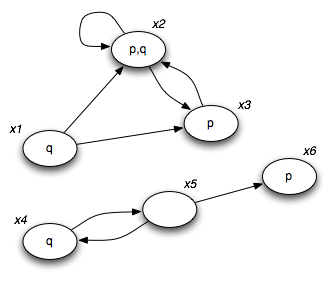
\includegraphics[width=0.65\textwidth]{./Images/Kripke01.png}
  	\caption{Beispiel einer Kripke-Struktur}
		\label{fig:mmKripke01}
	\end{center}
\end{figure}

\begin{definition}
	\label{def:reasoning}
	Sei $M = (W,R,L)$ ein Model einer Modal Logik und $\phi$ sei eine Formel nach \eqref{eqn:bnf}.
	Dann lässt sich nach folgenden Regeln schließen ob $\phi$ in einer Welt $x$ \emph{Wahr} oder \emph{Falsch} ist.
	\begin{align}
	%	\begin{split}
		x &\Vdash \top\label{eqn:semanticTrue}\\
		x &\nVdash \bot\label{eqn:semanticFalse}\\
		x &\Vdash p\text{ gdw. }p \in L(x)\label{eqn:semanticLabel}\\
		x &\Vdash \neg \phi\text{ gdw. }x \nVdash \phi\\
		x &\Vdash \phi \wedge \psi\text{ gdw. }x \Vdash \phi\text{ und } x \Vdash \psi\label{eqn:semanticAnd}\\
		x &\Vdash \phi \vee \psi\text{ gdw. }x \Vdash \phi \text{, oder } x \Vdash \psi\\
		x &\Vdash \phi \rightarrow \psi\text{ gdw. }x \Vdash \psi\text{, immer wenn gilt }x \Vdash \phi\\
		x &\Vdash \phi \leftrightarrow \psi\text{ gdw. }( x \Vdash \phi\text{ gdw. }x \Vdash \psi)\label{eqn:semanticBiconditional}\\
		x &\Vdash \Box \psi \text{ gdw. }\forall y \in W \text{ gilt } R(x,y)\text{, und } y \Vdash \psi\label{eqn:semanticBox}\\
		x &\Vdash \Diamond \psi\text{ gdw. }\exists y \in W \text{ sodass }R(x,y)\text{ und }y \Vdash \psi\label{eqn:semanticDiamond}
	%	\end{split}
	\end{align}	
\end{definition}
\cite[S.310]{huth2004logic}\\
\\
%
%
Die Formeln \eqref{eqn:semanticTrue} und \eqref{eqn:semanticFalse} besagt, dass die Werte \true und \false enthalten sind. 

Die Formel \eqref{eqn:semanticLabel} besagt, dass wir Aussagen folgern können die Teil der Wissensbasis sind.

Die Formeln \eqref{eqn:semanticAnd} bis \eqref{eqn:semanticBiconditional} sind ähnlich zu denen aus der Aussagenlogik.

Besonders zu beachten sind die Formeln \eqref{eqn:semanticBox} und \eqref{eqn:semanticDiamond}. 
\eqref{eqn:semanticBox} besagt, dass die Aussage $\Box\psi$ für eine Welt $x$ gefolgert werden kann, wenn diese in allen Welten die von $x$ aus erreichbar sind, folgerbar ist. 
Dies beinhaltet $x$ nur wenn $R(x,x)$ gilt.
Wichtig ist das die Aussage lediglich fordert, das eine Aussage in allen \emph{erreichbaren} Welten gefolgert werden kann. $x \Vdash \Box \bot$ ist also \true wenn $x$ mit keiner anderen Welt verbunden ist.

Die Formel \eqref{eqn:semanticBox} ist ähnlich, nur das sie einen Existenz-Charakter hat. 
Aus $x$ lässt sich $\Diamond \psi$ folgern, wenn es min. eine Welt gibt die von $x$ erreichbar ist, in der sich $\psi$ folgern lässt. 
Wichtig ist die Aussage \emph{es existiert} eine Welt. 
$x \Vdash \Diamond \top$ ist also \false wenn es keine Welt $x'$ gibt für die gilt $R(x,x')$.\\


\begin{figure}
	\centering
	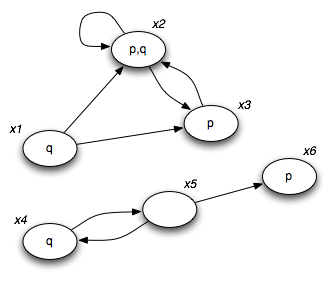
\includegraphics[height=6.5cm]{Images/Kripke01.png}
	\caption{Kripke Model Beispiel für Model Folgerungsbeispiele}
	\label{fig:Kripke01}
\end{figure}


\begin{definition}
	\label{def:model_erfuellt}
	Ein Model $\mathcal{M}$ einer Modal Logik erfüllt eine Formel $\phi$ wenn jeder Zustand im Model die Formel erfüllt.
	Wir schreiben für diesen Fall $\mathcal{M} \vDash \psi$ gdw. $\forall x \in W, x \Vdash \psi$ gilt.
\end{definition}
\cite[S.310f]{huth2004logic}
%
Anhand des Kripke Models \Abb{Kripke01} werden nun ein paar Beispielformeln diskutiert um die Definitionen zu konkretisieren:

\curr
\begin{itemize}
	\item $x_1 \vDash q$, gilt wegen $q \in L(Lx_1)$
	\item $x_1 \vDash \Diamond q$, weil es einen erreichbare Welt (hier $x_2$) $q \in L(x_2)$ gilt. Mathematisch formuliert: es gilt $R(x_1, x_2)$ und $x_2 \vDash q$
	\item $x_1 \nvDash \Box q$, weil $R(x_1,x_3)$ und $x_3 \nvDash q$. $\Box$ setzt voraus, dass \emph{alle} erreichbaren Welt die Bedingung erfüllen.
	\item $x_5 \nvDash \Box p$ und $x_5 \nvDash \Box q$ sogar $x_5 \nvDash \Box p \vee \Box q$, allerdings gilt $x_5 \vDash \Box (p \vee q)$. $x_5 \nvDash \Box p$ gilt, weil $x_4$ erreichbar ist, aber nicht $p$ enthält. $x_5 \nvDash \Box q$ gilt weil, $x_6$ erreichbar ist aber kein $q$ enthält. Damit gilt auch $x_5 \nvDash \Box p \vee \Box q$. $x_5 \vDash \Box (p \vee q)$ gilt hingegen, weil alle erreichbaren Welten $(x_5, x_6)$ entweder $p$ oder $q$ enthalten.
	\item Die Welten die $\Box p \rightarrow p$ erfüllen sind: $x_2, x_3, x_4, x_5, x_6$.
	Die Welten $x_2, x_3, x_6$ erfüllend die Formeln mit \true, weil sei $p$ enthalten und $\Box p$ gilt. Für $x_6$ gilt $\Box q$ weil es keine erreichbaren Welten hat (vgl. Formel \eqref{eqn:semanticBox} ).
	Die Welten $x_4, x_5$ erfüllen die Formel mit \false, weil sie $p$ nicht enthalten und nicht alle von ihnen erreichbaren Welten $p$ enthalten. $x_5 \nvDash \Box p$ ist der Fall, weil $x_4$ zutrifft.
\end{itemize}
%
Welten wie $x_6$ die keine Verbindungen zu anderen Welten erfordern besonderes Augenmerk.
Die Formel $x_6 \nvDash \Diamond \phi$ gilt z.B. immer, auch wenn $\phi = \top$ weil $\Diamond$ min eine verbundene Welt voraussetzt.
$x \nvDash \Diamond \top$ gilt z.B. immer wenn $x$ min. eine erreichbare Welt hat, weil $\top$ per Definition in jeder Welt erfüllt ist.
Ähnlich verhält es sich mit $x_6 \vDash \Box \phi$. Diese Aussage gilt immer egal welchen Wert $\phi$ besitzt.
Das gilt auch für die Aussage $x_6 \Vdash \Box \bot$. 
Auch wenn $\bot$ per Definition in jeder Welt \false ist, ist die Aussage $x_6 \Vdash \Box \bot$ \true, wenn es keine anderen verbundenen Welten gibt.
Es ist schlicht weg nicht möglich das Gegenteil zu beweisen, weil es keine Gegenbeispiele geben kann.
Auch wenn diese Interpretationen nicht intuitiv sind, sichern die sie die Morgen Bedingung siehe \eqref{eqn:semanticBox}



%
%
\paragraph{\formelSchemata} % (fold)
\label{par:formel_schemata}
\formelSchemata beschreiben eine generelle Form, ein Pattern, von Formeln.
Ihr \parseTree ist unvollständig, an jedem Blatt ist platz für eine weitere valide \ML Formel.
Jede Belegung eines solchen \formelSchema wird \fachwort{Instanz} genannt.
Die Anzahl der möglichen Instance ist unendlich.\\
\\
Hier ein paar Instanzen-Beispiele für das \formelSchema $\psi \rightarrow \Box \Diamond \psi$:\\
\begin{itemize}
	\item $p \rightarrow \Box \Diamond p$
	\item $q \rightarrow \Box \Diamond q$
	\item $(p \wedge r \rightarrow q) \rightarrow \Box \Diamond (p \wedge r \rightarrow q)$
\end{itemize}

% paragraph formel_schemata (end)

\textbf{Gleichheit zwischen modal logischen Formeln}
\begin{definition}
	\label{def:model_folgert}
	\begin{itemize}
		\item Eine Menge von modal logischen Formeln $\Gamma$ folgert eine modal logische Formel $\psi$, gdw. wenn für jede Welte $w$ aus jedem Model $\mathcal{M}$ gilt $x \Vdash \psi$ immer wenn gilt $x \Vdash \phi$ $\forall \phi \in \Gamma$. 
		Dies wird notiert durch $\Gamma \vDash \psi$.
		\item Wir bezeichnen zwei modal logische Formeln $\phi$ und $\psi$ als semantisch äquivalente wenn sowohl $\psi \vDash \phi$ als auch $\psi \vDash \phi$ gilt und notieren dies mit $\psi \equiv \phi$.
	\end{itemize}	
\end{definition}
\cite[S.313]{huth2004logic}


\begin{equation}
	\neg \Box \phi \equiv \Diamond \neg \phi \text{ und } \neg \Diamond \phi \equiv \Box \neg \phi
\end{equation}


\textbf{valide Formeln}
\begin{definition}
	\label{def:valide}
	Eine modal logische Formel $\psi$ wird valide genant wenn sie in jeder Welt in jedem Model \emph{Wahr} ist, also gdw. $\vDash \psi$ gilt.
\end{definition}
\cite[S.314]{huth2004logic}

Dadurch das man bestimme Formeln als valide voraussetzt, kann man eigene Logiken und damit andere modale von \true erzeugen.
Die \NML $K$ schreibt nur die Validität der Formel \KFormel vor.
Diese bewirkt, dass \todo{Wirkung eintragen}.\\
Im nächsten Kapitel werden weitere Formeln, die als valide vorausgesetzt werden können, vorgestellt und deren Auswirkungen diskutiert.







% section semantik (end)
